\subsection{Casos de test}

% Evaluamos\footnote{El script asociada se puede encontrar en \textit{./experimentos/tiempo_ejecucion.py}, los archivos resultado en \textit{./experimentos/resultados/tiempo-de-ejecucion}} el error absoluto en norma $L_1$ de los resultados de nuestra implementación de PageRank sobre el \textit{método de Jacobi} y el \textit{método de Gauss-Seidel} para los casos no triviales de test provistos por la cátedra\footnote{Los mismos se pueden encontrar en \textit{./catedra/tests-pagerank}}, en función de la cantidad de iteraciones realizadas.

Notamos que las matrices asociadas a la resolución de \textit{PageRank} son estocásticas en columna, por lo que ambos métodos siempre convergerán a una solución\footnote{Damos una demostración informal de este hecho: se puede demostrar que los métodos propuestos convergen para matrices estrictamente diagonal dominantes. En consecuencia, las matrices de iteración asociadas deben tener radio espectral $<$ 1. Como las matrices estocásticas en columna son la traspuesta de las matrices estrictamente diagonal dominantes y los autovalores de una matriz equivalen a los de su traspuesta, entonces debe ser que las matrices de iteración asociadas a las matrices estocásticas en columna tienen radio espectral $<$ 1. Como además su diagonal es no nula, entonces satisfacen las condiciones de convergencia para los métodos iterativos mencionados.}. 

\vspace{2em}
\noindent\textsc{Metodología}. Se evaluó el error absoluto $||x - pagerank(g,\ p)||_1$, donde $x$ refiere a la solución verdadera, $g$ refiere al grafo de entrada y $p$ al \textit{valor p}\footnote{Para una explicación en más detalle de PageRank, ver el $tp1$.}, para cada caso de test provisto, en función de la cantidad de iteraciones $q$ a realizar en el rango $[1, 100]$.

Se repitió el experimento para dos implementaciones del algoritmo que difieren unicamente en el método de resolución del sistema lineal asociado a $PageRank$. En la primera se utilizó el \textit{método de Jacobi} y en la segunda el \textit{método de Gauss-Seidel}. Se controló la tolerancia ($t = 0$) para forzar a los algoritmos a iterar de manera exacta. 

\vspace{2em}
\noindent\textsc{Resultados}. Las figuras (\ref{test_15_segundos}.) a (\ref{test_trivial}.) muestran los los resultados del error absoluto $L_1$ para cada caso de test.

\vspace{1em}
Notamos que la implementación de \textit{PageRank} sobre el \textit{método de Gauss-Seidel} tuvo una velocidad de convergencia mayor a la que logró la implementación sobre el \textit{método de Jacobi}. 

\vspace{1em}
Además, para éste primer método, bastó $q < 60$ para lograr un error absoluto $L_1$ menor a $10^{-6}$ para todos los casos de test. En cambio, el \textit{método de Jacobi} requirió más iteraciones ---para alcanzar la misma meta--- en un sólo caso: el test \textit{15\_segundos}. En particular, para este caso y el test \textit{30\_segundos}, notamos que la cantidad de iteraciones requeridas para converger no parece depender de manera estricta del tamaño de la matriz, pero sí parece existir una correlación.

\vspace{1em}
Consideramos, también, que la meseta de error observado por debajo de $10^{-6}$ debe corresponder a un error de redondeo entre las soluciones esperadas y las computadas durante el experimento. Sin embargo, observamos que esta meceta no ocurre, en particular, en el test \textit{completo}.

%\vspace{1em}
%Sin embargo, dadas las limitaciones de esta evaluación ---en particular la poca representatividad de los casos de test---, poco se puede decir respecto al corportamiento general de ambos métodos. 

%\vspace{1em}
\begin{figure}[!htbp]
    %\ContinuedFloat
    \centering
    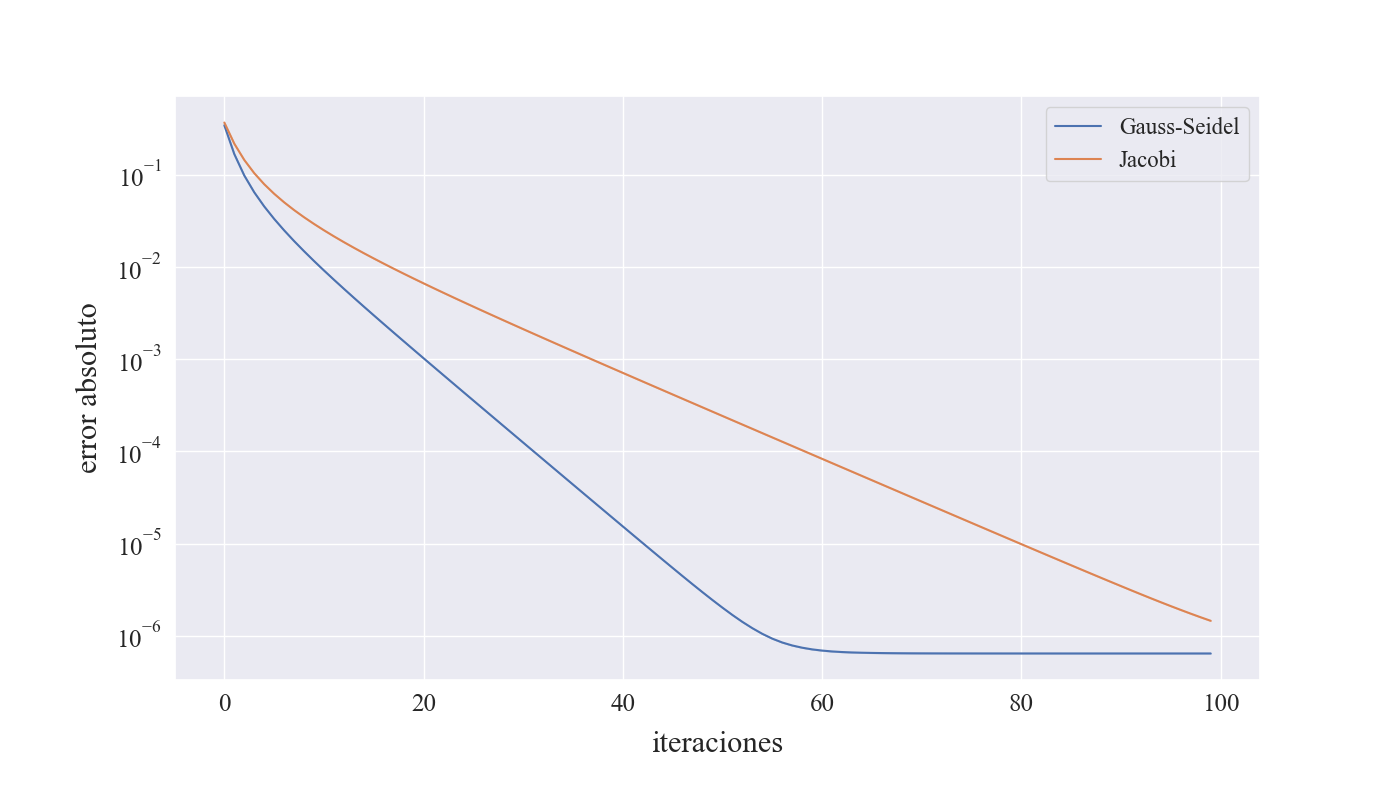
\includegraphics[width=1\textwidth, trim=0 0 0 30]{files/src/.media/convergencia_test_15_segundos.png}
    \caption{Error absoluto $L_1$ para el grafo del test \textit{15\_segundos}, con $n = 2000$ y $p = 0.9$, en función de la cantidad de iteraciones realizadas, para ambas implementaciones de pagerank.} \label{test_15_segundos}
\end{figure}

%\vspace{1em}
\newpage
\begin{figure}[!htbp]
    %\ContinuedFloat
    \centering
    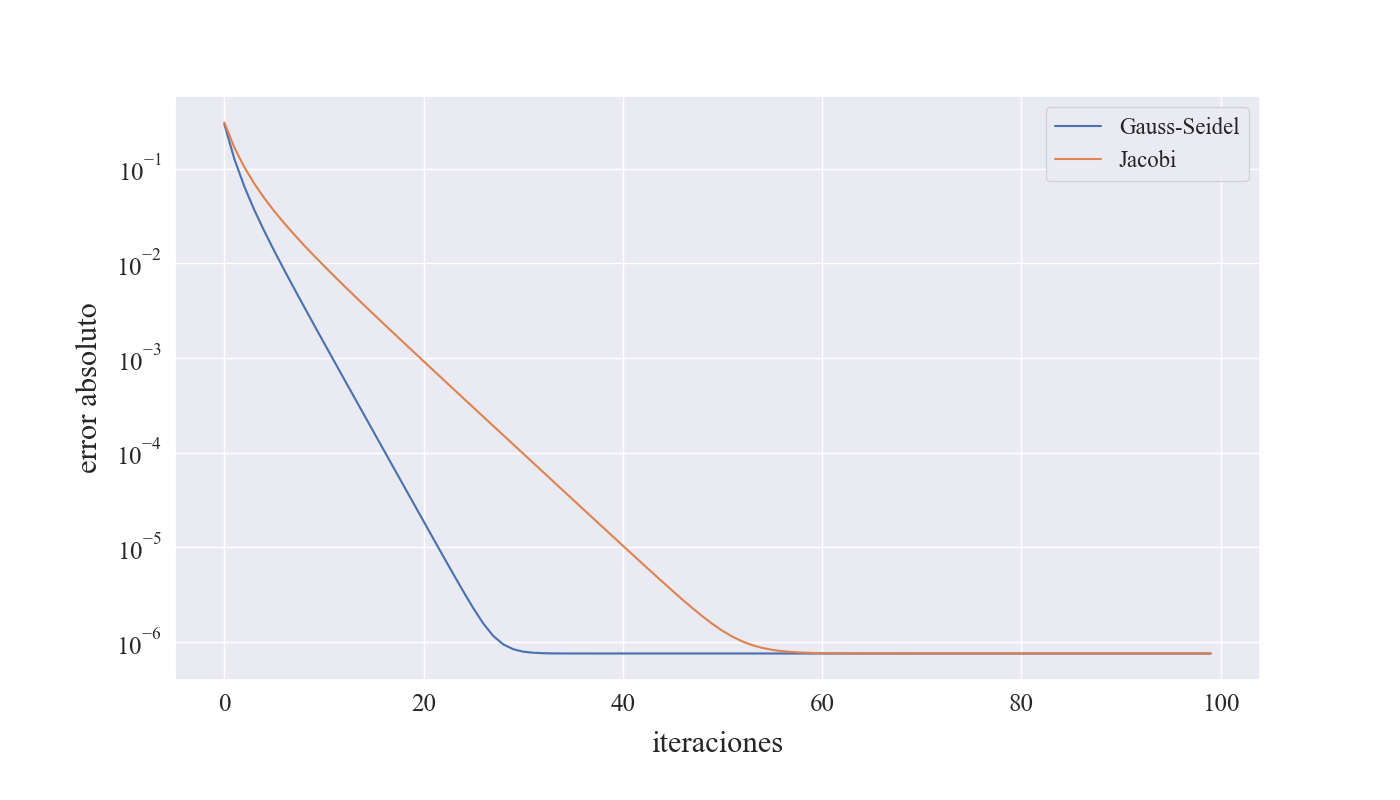
\includegraphics[width=1\textwidth, trim=0 0 0 10]{files/src/.media/convergencia_test_30_segundos.png}
    \caption{Error absoluto $L_1$ para el grafo del test \textit{30\_segundos}, con $n = 3000$ y $p = 0.8$, en función de la cantidad de iteraciones realizadas, para ambas implementaciones de pagerank.} \label{test_30_segundos}
\end{figure}

%\vspace{1em}
\begin{figure}[!htbp]
    %\ContinuedFloat
    \centering
    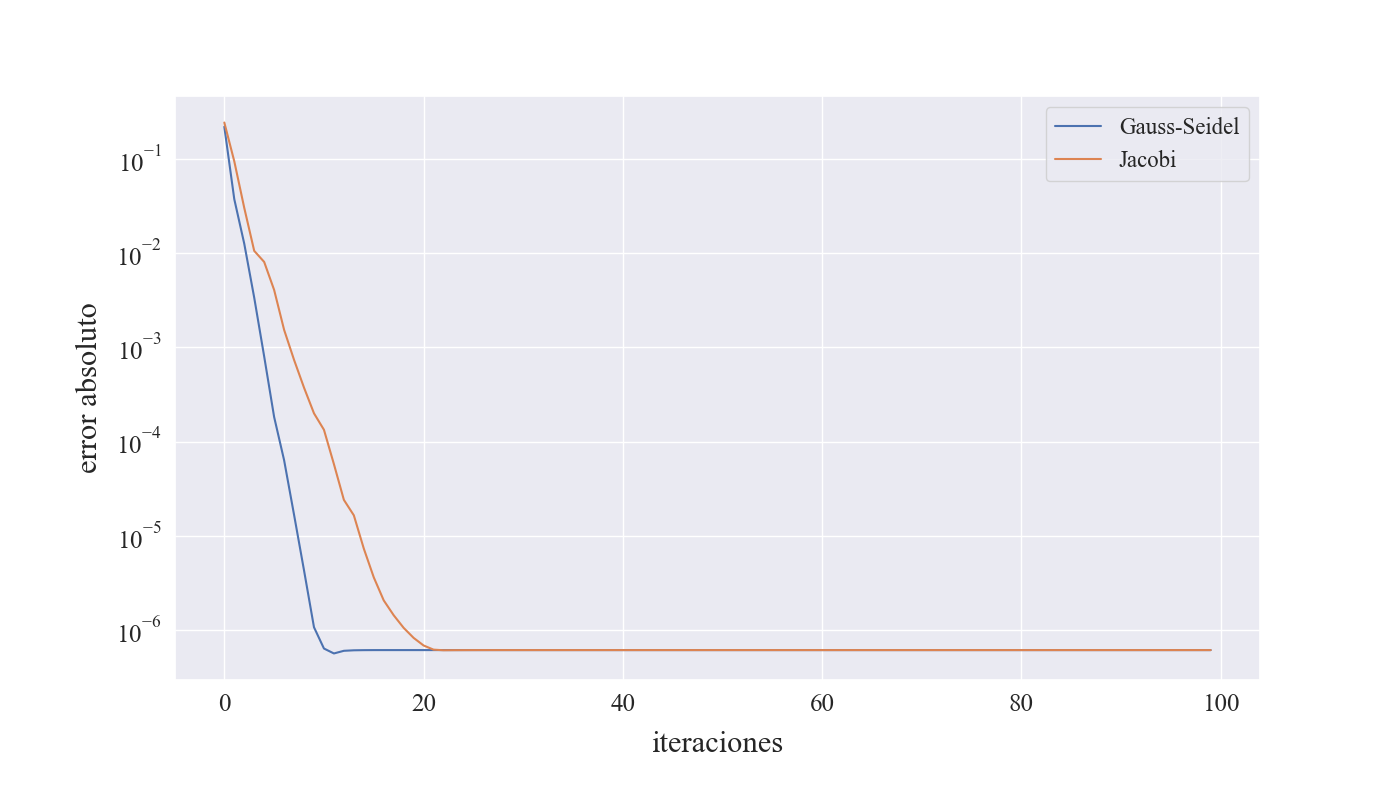
\includegraphics[width=1\textwidth, trim=0 0 0 30]{files/src/.media/convergencia_test_aleatorio_desordenado.png}
    \caption{Error absoluto $L_1$ para el grafo del test \textit{aleatorio\_desordenado}, con $n = 5$ y $p = 0.76$, en función de la cantidad de iteraciones realizadas, para ambas implementaciones de pagerank.} \label{test_aleatorio_desordenado}
\end{figure}

%\vspace{1em}
\begin{figure}[!htbp]
    %\ContinuedFloat
    \centering
    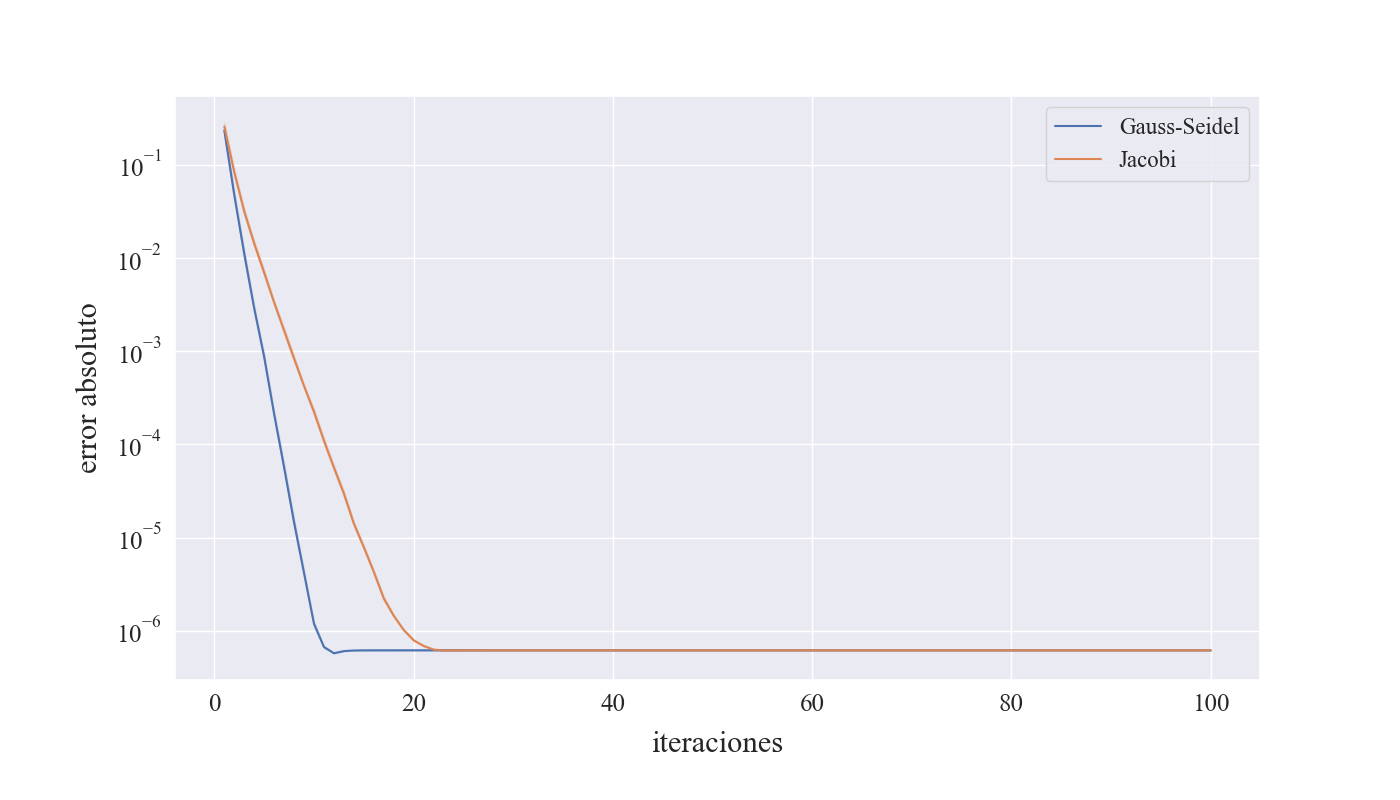
\includegraphics[width=1\textwidth]{files/src/.media/convergencia_test_aleatorio.png}
    \caption{Error absoluto $L_1$ para el grafo del test \textit{aleatorio}, con $n = 5$ y $p = 0.76$, en función de la cantidad de iteraciones realizadas, para ambas implementaciones de pagerank.} \label{test_aleatorio}
\end{figure}

%\vspace{1em}
\begin{figure}[!htbp]
    %\ContinuedFloat
    \centering
    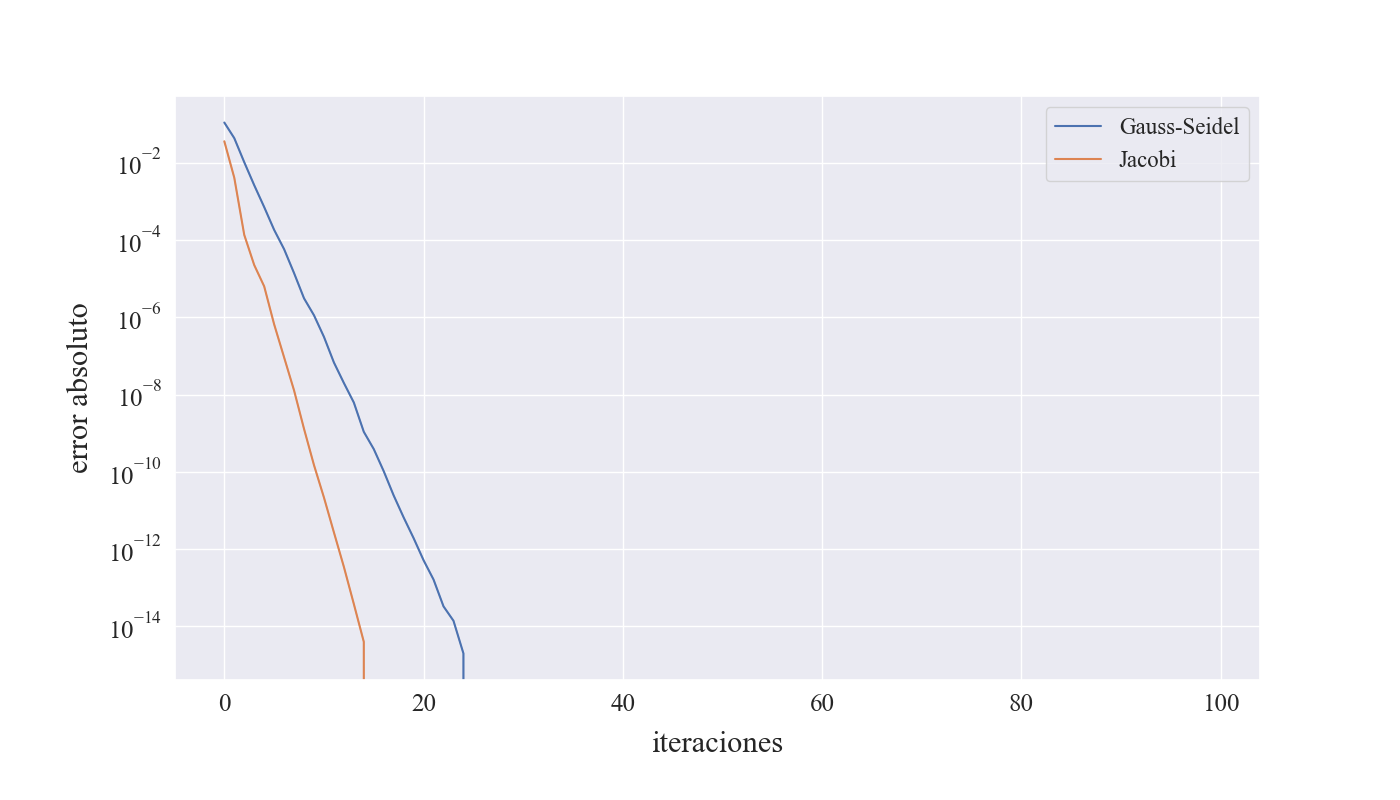
\includegraphics[width=1\textwidth]{files/src/.media/convergencia_test_completo.png}
    \caption{Error absoluto $L_1$ para el grafo del test \textit{completo}, con $n = 5$ y $p = 0.5$, en función de la cantidad de iteraciones realizadas, para ambas implementaciones de pagerank.} \label{test_completo}
\end{figure}

%\vspace{1em}
\begin{figure}[!htbp]
    %\ContinuedFloat
    \centering
    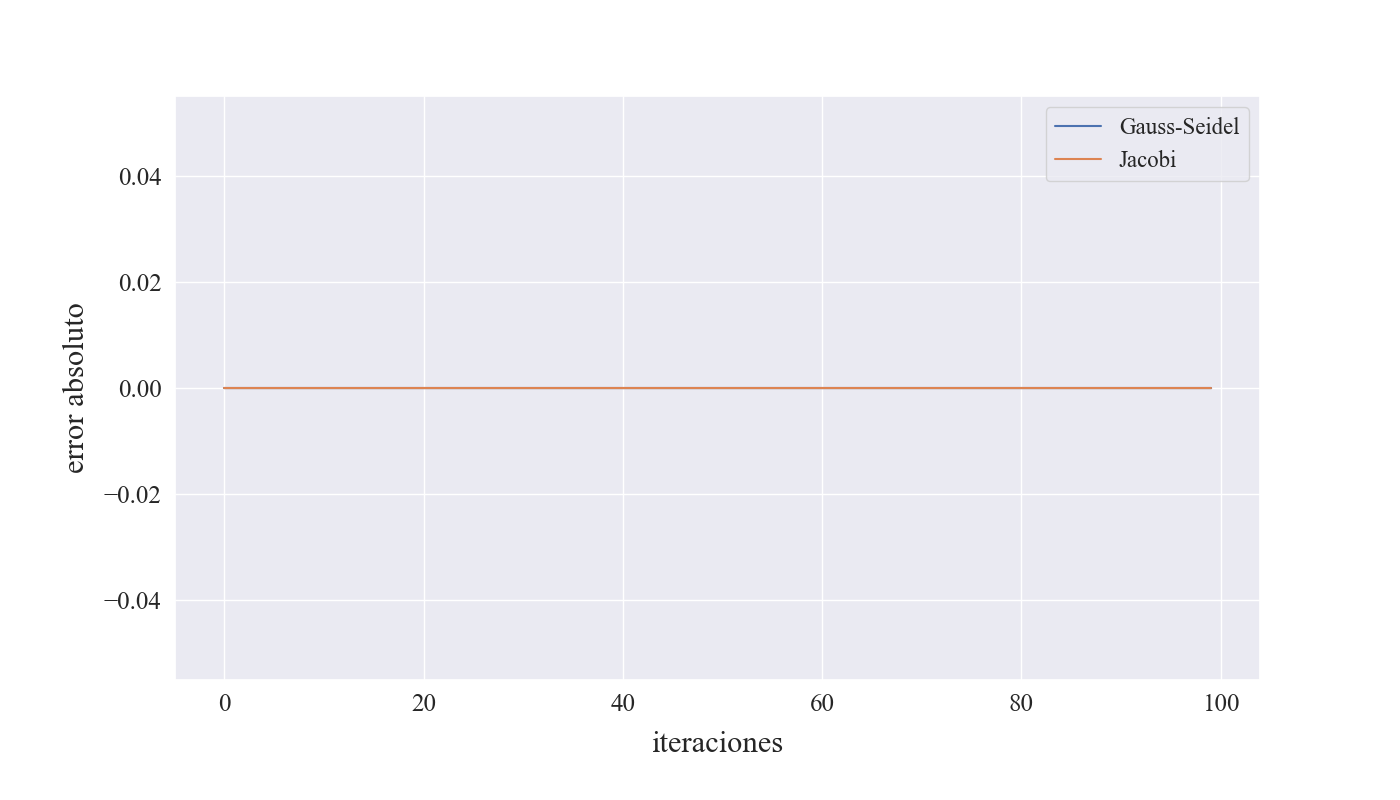
\includegraphics[width=1\textwidth]{files/src/.media/convergencia_test_sin_links.png}
    \caption{Error absoluto $L_1$ para el grafo del test \textit{sin\_links}, con $n = 5$ y $p = 0.64$, en función de la cantidad de iteraciones realizadas, para ambas implementaciones de pagerank.} \label{test_sin_links}
\end{figure}

%\vspace{1em}
\begin{figure}[!htbp]
    %\ContinuedFloat
    \centering
    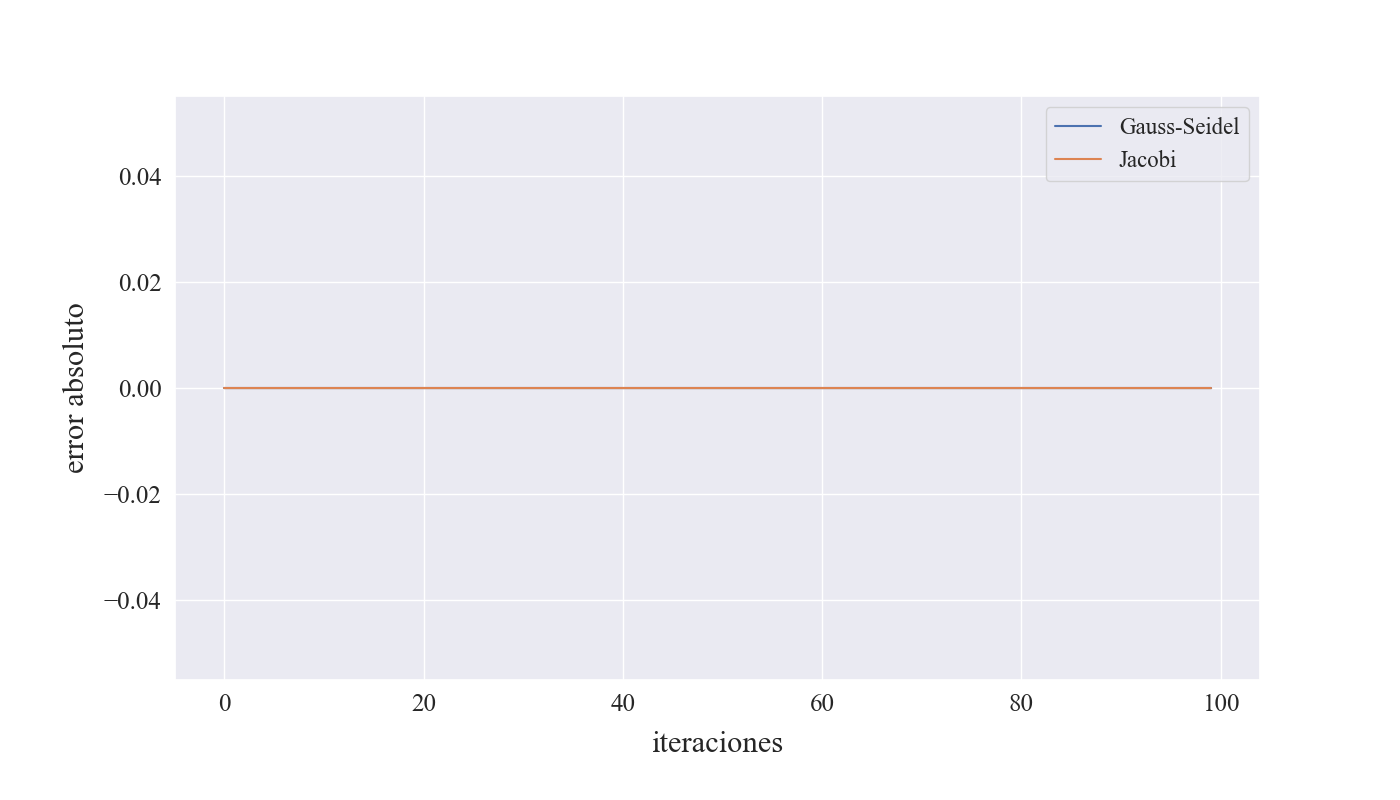
\includegraphics[width=1\textwidth]{files/src/.media/convergencia_test_trivial.png}
    \caption{Error absoluto $L_1$ para el grafo del test \textit{trivial}, con $n = 1$ y $p = 0.3$, en función de la cantidad de iteraciones realizadas, para ambas implementaciones de pagerank.} \label{test_trivial}
\end{figure}

\vspace*{1em}
Procedemos a mostrar los resultados finales para el error absoluto con norma $L_1$ y $L_{\infty}$ ---para hacer una comparación por coordenadas---, tras las cien iteraciones:

\vspace{1em}
\begin{figure}[!htbp]
        \begin{tabular}{ |c|c|c|c|c|c|c| } 
        \hline
                                & \multicolumn{2}{c|}{Jacobi}    & \multicolumn{2}{c|}{Gauss-Seidel} \\
        \hline
        test                    & $L_1$             & $L_{\infty}$      & $L_1$     & $L_{\infty}$ \\
        \hline
        15\_segundos            & $1.45 \times 10^{-6}$  & $9.76 \times 10^{-9}$  & $6.4 \times 10^{-7}$  & $5 \times 10^{-9}$ \\
        30\_segundos            & $7.54 \times 10^{-7}$  & $5 \times 10^{-10}$  & $7.54 \times 10^{-7}$  & $5 \times 10^{-10}$ \\
        aleatorio\_desordenado   & $6.18 \times 10^{-6}$  & $2.52 \times 10^{-7}$  & $6.18 \times 10^{-7}$  & $2.52 \times 10^{-7}$ \\
        aleatorio               & $6.18 \times 10^{-6}$  & $2.52 \times 10^{-7}$  & $6.18 \times 10^{-7}$  & $2.52 \times 10^{-7}$ \\
        completo                & $0$  & $0$  & $0$  & $0$ \\
        sin\_links              & $0$  & $0$  & $0$  & $0$ \\
        trivial                 & $0$  & $0$  & $0$  & $0$ \\
        \hline                  
        \end{tabular}       
    \bigskip
    \caption{Error absoluto $L_1$ y $L_{\infty}$ de los casos de test para las implementaciones de $PageRank$ sobre los métodos de \textit{Jacobi} y \textit{Gauss-Seidel}.} \label{convergencia_resultados}
\end{figure}
